% Provenance (never printed): old premiere S material on the oceanic lithosphere
% (ophiolite-type layering, peridotite and gabbro, partial melting by decompression
% at the ridge, hydrothermalism, cooling and subsidence of the lithosphere with
% age); see sources/book2/PROVENANCE.md. Melting from figdata/grade-11/
% ridge_melting.py (adiabat and Hirschmann solidus), depth against age from
% depth_age.py (ETOPO1 and the Seton 2020 age grid). Partial melting is re-founded
% in Year 2 (mantle-melting); fault is Book 1's (g7), normal fault is defined here.
\chapter{महासागरीय कटक और महासागरीय स्थलमंडल}\label{ch:g11:ocean-ridges}

फ़रवरी 1977 में पूर्वी प्रशांत में गैलापागोस दरार के ऊपर 2500 मीटर नीचे
खींची जा रही एक कैमरा-स्लेज ने कटक के नंगे काले लावा के एक के बाद एक
चित्र लिए। फिर उसके तापमापी ने जल के तापमान में एक छोटी वृद्धि दर्ज की,
और चित्रों पर लावा
सैकड़ों सफ़ेद सीपियों से ढका था। कुछ दिन बाद पनडुब्बी \emph{ऐल्विन}
दो भूवैज्ञानिकों को उस स्थान तक नीचे ले गई: लावा की दरारों से गरम, झिलमिलाता जल
बाहर बह रहा था, और उसके चारों ओर अग्रबाहु जितनी लंबी सीपियाँ,
शंबुक और सफ़ेद केकड़े रहते थे; बाद के एक गोते में लाल सिरों वाले नलिका-कृमि भी। किसी ने
वहाँ जीवन की अपेक्षा नहीं की थी, इसलिए जहाज़ पर कोई जीवविज्ञानी नहीं था। यह अध्याय समझाता है
कि भूवैज्ञानिकों ने क्या पाया था: कटकों पर महासागरीय तली कैसे बनती है,
वहाँ वह गरम क्यों है, और दूर जाते हुए उसका क्या होता है।
% ledger: whoi:alvin-1977

\begin{recall}
कटकों पर नई महासागरीय तली बनती है और दोनों ओर दूर चलती है, जिससे
उसकी आयु अक्ष से दूरी के साथ बढ़ती है; कटक लगभग
\qty{65000}{km} लंबा एक तंत्र बनाते हैं, धीमे कटकों के अनुदिश एक भ्रंश घाटी के साथ और तेज़ कटकों के अनुदिश
एक चिकने शिखर के साथ (\cref{ch:g11:drift-to-spreading})। प्लेटें किसी कटक के आर-पार
प्रति वर्ष कुछ सेंटीमीटर की दर से एक-दूसरे से दूर होती हैं, मध्य-अटलांटिक कटक की अपेक्षा
पूर्वी प्रशांत उभार के आर-पार अधिक तेज़ी से (\cref{ch:g11:plate-motions})। \omterm{def:g11:lithosphere-asthenosphere:lithosphere}{स्थलमंडल}
कठोर बाहरी कवच है, उसके नीचे का \omterm{def:g11:lithosphere-asthenosphere:lithosphere}{दुर्बलतामंडल} बहता है; \omterm{def:g11:lithosphere-asthenosphere:lithosphere}{दुर्बलतामंडल} का तापमान
गहराई के प्रति किलोमीटर केवल लगभग \qty{0.45}{\celsius} बढ़ता है,
और प्रावार की चट्टान का गलनांक गहराई के साथ बढ़ता है
(\cref{ch:g11:lithosphere-asthenosphere})। मैग्मा सतह के नीचे की पिघली चट्टान है,
बेसाल्ट वह गहरे रंग की चट्टान जो लावा ठंडा होने पर बनाता है, और भ्रंश ऐसी
दरार जिसके अनुदिश चट्टानें खिसकी हैं (पुस्तक 1, कक्षा 6 और 7)।
\end{recall}
% ledger: noaa:ridge, katsura10:adiabat, hirschmann:solidus

\section{महासागरीय स्थलमंडल}

महाद्वीपों की सतह पर दुर्लभ दो चट्टानें
\omterm{def:g11:ocean-ridges:oceanic-lithosphere}{महासागरीय स्थलमंडल} का अधिकांश भाग बनाती हैं।

\begin{definition}[पेरिडोटाइट]\label{def:g11:ocean-ridges:peridotite}
\emph{पेरिडोटाइट}\index{पेरिडोटाइट} एक गहरे रंग की, मोटे कणों वाली चट्टान है जो
मुख्यतः खनिज ओलिवीन से बनी है, कुछ पाइरॉक्सीन के साथ। यह प्रायः हरी और
घनी होती है। माना जाता है कि पृथ्वी के प्रावार का अधिकांश भाग पेरिडोटाइट से बना है।
\end{definition}

\begin{definition}[गैब्रो]\label{def:g11:ocean-ridges:gabbro}
\emph{गैब्रो}\index{गैब्रो} एक गहरे रंग की, मोटे कणों वाली आग्नेय चट्टान है जो
मुख्यतः प्लेजियोक्लेज़ फ़ेल्डस्पार और पाइरॉक्सीन से बनी है। इसका संघटन
बेसाल्ट जैसा ही है, पर यह भूमि के गहरे भीतर धीरे-धीरे क्रिस्टलित हुई, जिससे इसके क्रिस्टलों को
बढ़ने का समय मिला। यह गहरी \omterm{def:g11:ocean-ridges:oceanic-lithosphere}{महासागरीय भूपर्पटी} की सबसे प्रचुर चट्टान है।
\end{definition}
% ledger: geo:peridotite, geo:gabbro

यहाँ नामित खनिजों, ओलिवीन, पाइरॉक्सीन और फ़ेल्डस्पार, का वर्णन
\cref{ch:g11:minerals} में है।

\begin{omfigure}
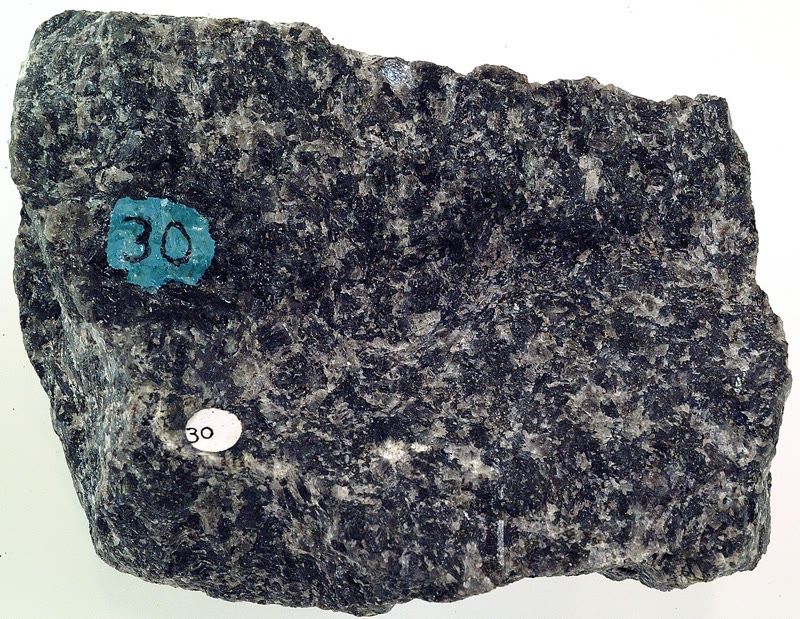
\includegraphics[height=4.2cm]{images/book2/g11-geodil-gabbro.jpg}\hspace{0.03\linewidth}%
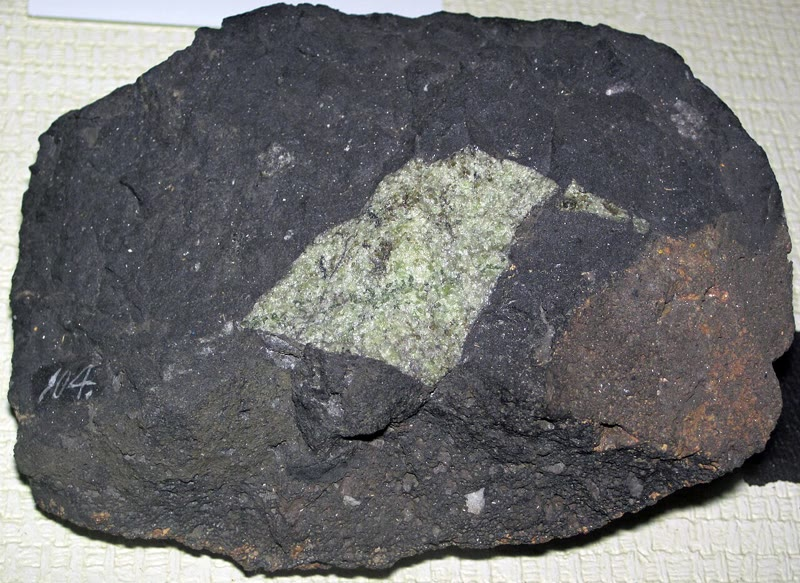
\includegraphics[height=4.2cm]{images/book2/g11-stjohn-peridotite.jpg}

{\small बाएँ: \omterm{def:g11:ocean-ridges:gabbro}{गैब्रो}, \qty{9}{cm} चौड़ा, गहरे पाइरॉक्सीन और हल्के
फ़ेल्डस्पार के इतने बड़े क्रिस्टलों के साथ कि वे दिख जाते हैं; फ़ोटो डार्ला सोंड्रोल (CC0)।
दाएँ: प्रावार से आया हरे \omterm{def:g11:ocean-ridges:peridotite}{पेरिडोटाइट} का एक ढेला, जो एरिज़ोना के एक ज्वालामुखी के
काले बेसाल्ट लावा के भीतर ऊपर लाया गया; फ़ोटो जेम्स सेंट~जॉन (CC~BY~2.0)।}
\end{omfigure}
% ledger: photo:g11-gabbro, photo:g11-peridotite

\begin{definition}[महासागरीय भूपर्पटी; महासागरीय स्थलमंडल]\label{def:g11:ocean-ridges:oceanic-lithosphere}
\emph{महासागरीय भूपर्पटी}\index{महासागरीय भूपर्पटी} महासागर की तली की
भूपर्पटी है: लगभग \qty{7}{km} बेसाल्ट और \omterm{def:g11:ocean-ridges:gabbro}{गैब्रो}, जो कटकों पर बनती है।
\emph{महासागरीय स्थलमंडल}\index{महासागरीय स्थलमंडल} महासागरीय भूपर्पटी
और उसके नीचे के सबसे ऊपरी प्रावार का कठोर \omterm{def:g11:ocean-ridges:peridotite}{पेरिडोटाइट}, दोनों मिलकर, है।
\end{definition}

पूरे महासागरों के भूकंपीय सर्वेक्षण \omterm{def:g11:ocean-ridges:oceanic-lithosphere}{महासागरीय भूपर्पटी} को, विभंग-क्षेत्रों और तप्त स्थलों से दूर,
\qty{7.1}{km} की औसत मोटाई देते हैं, \qty{0.8}{km} कम-ज़्यादा। इसकी परतें गहरे वेधन से और
महाद्वीपों पर ऊपर धकेली गई पुरानी महासागरीय तली के टुकड़ों से ज्ञात हैं। 2005 में एक वेधन-जहाज़
ने पूर्वी प्रशांत की 15 मिलियन वर्ष पुरानी भूपर्पटी में \qty{1507}{m} गहरा
छेद पूरा किया, जो लावाओं से, डाइकों से होते हुए,
\omterm{def:g11:ocean-ridges:gabbro}{गैब्रो} तक जाने वाला पहला छेद था:
% ledger: white92:crust, iodp1256:section, geo:peridotite

\begin{itemize}
  \item शीर्ष पर \emph{अवसादों} का एक पतला आवरण, जो कटक-अक्ष पर
        अनुपस्थित है और पुरानी तली पर अधिक मोटा;
  \item \qty{800}{m} से अधिक \emph{बेसाल्ट लावा}, जो समुद्री तल पर
        चादरों के रूप में और \emph{तकियों} के रूप में फूटे --- काँच जैसी खाल वाली
        लावा की गोल नलियाँ और लोंदे;
  \item \emph{चादरी डाइक}, इस छेद में \qty{346}{m}: बेसाल्ट की सैकड़ों
        ऊर्ध्वाधर चादरें, हर एक वह जमी हुई दरार जिससे होकर मैग्मा
        किसी उद्गार तक उठा था, किताब के पन्नों की तरह साथ-साथ;
  \item \emph{\omterm{def:g11:ocean-ridges:gabbro}{गैब्रो}}, जो समुद्री तल से \qty{1407}{m} नीचे मिला, वह मैग्मा
        जो डाइकों के नीचे, \omterm{def:g11:seismic-structure:moho}{मोहो} तक, धीरे-धीरे क्रिस्टलित हुआ;
  \item \omterm{def:g11:seismic-structure:moho}{मोहो} के नीचे प्रावार का \emph{\omterm{def:g11:ocean-ridges:peridotite}{पेरिडोटाइट}}।
\end{itemize}
% ledger: iodp1256:section, geo:basalt-ridges, geo:gabbro

\begin{omfigure}
\begin{tikzpicture}[x=1cm, y=-0.55cm, font=\footnotesize]
% to scale in depth: lavas 0.8 km, dykes 0.35 km (iodp1256:section), crust 7.1 km (white92:crust)
  \fill[omLithAlluv] (0,-0.25) rectangle (2.4,0);
  \fill[lith basalt] (0,0) rectangle (2.4,0.8);
  \fill[omLithBasalt!60] (0,0.8) rectangle (2.4,1.15);
  \foreach \x in {0.15,0.35,...,2.3} \draw[black!55, line width=0.3pt] (\x,0.8) -- (\x,1.15);
  \fill[lith gabbro] (0,1.15) rectangle (2.4,7.1);
  \fill[lith peridotite] (0,7.1) rectangle (2.4,9.0);
  \draw (0,-0.25) rectangle (2.4,9.0);
  \draw[line width=0.9pt] (0,7.1) -- (2.4,7.1);
  \foreach \d in {0,2,4,6,8} {\draw (-0.1,\d) -- (0,\d); \node[anchor=east] at (-0.1,\d) {\d};}
  \node[rotate=90, anchor=south] at (-0.75,4.5) {समुद्री तल से नीचे गहराई (\unit{km})};
  \draw[black!60] (2.4,-0.13) -- (2.7,-1.0) -- (2.85,-1.0);
  \node[anchor=west] at (2.85,-1.0) {अवसाद};
  \draw[black!60] (2.4,0.4) -- (2.7,0.25) -- (2.85,0.25);
  \node[anchor=west] at (2.85,0.25) {लावा: तकिए और चादरी प्रवाह};
  \draw[black!60] (2.4,0.98) -- (2.7,1.6) -- (2.85,1.6);
  \node[anchor=west] at (2.85,1.6) {चादरी डाइक};
  \node[anchor=west] at (2.55,4.1) {गैब्रो};
  \node[anchor=west] at (2.55,7.1) {मोहो};
  \node[anchor=west] at (2.55,8.05) {प्रावार का पेरिडोटाइट};
  \draw[decorate, decoration={brace, amplitude=5pt}] (7.9,0) -- (7.9,7.1)
    node[midway, right=7pt, align=left] {महासागरीय भूपर्पटी\\लगभग \qty{7}{km}};
\end{tikzpicture}

{\small \omterm{def:g11:ocean-ridges:oceanic-lithosphere}{महासागरीय भूपर्पटी} की परतें, गहराई में पैमाने पर। लावाओं और डाइकों की
मोटाइयाँ पूर्वी प्रशांत में वेधित गहरे छेद की हैं;
कुल मोटाई भूकंपीय सर्वेक्षणों का औसत है। अवसाद का आवरण
तली की आयु के साथ अधिक मोटा होता जाता है।}
\end{omfigure}
% ledger: iodp1256:section, white92:crust

\begin{omfigure}
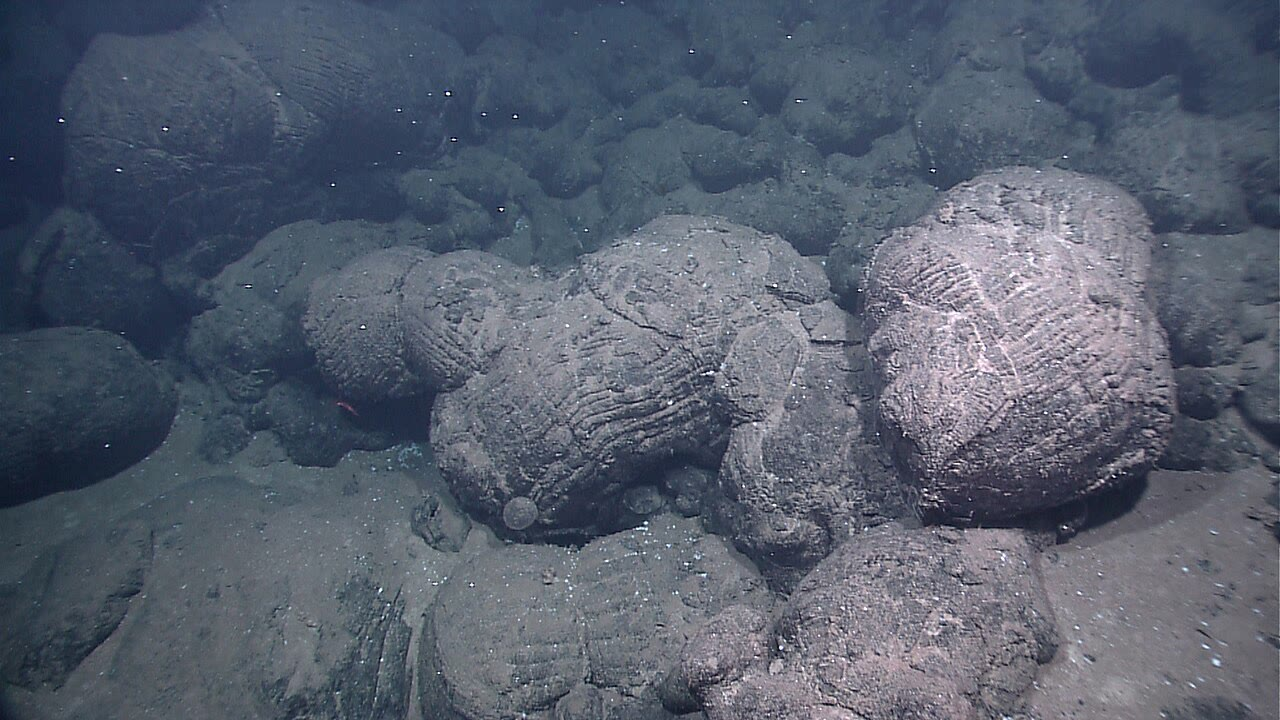
\includegraphics[width=0.8\linewidth]{images/book2/g11-noaa-pillow-lava.jpg}

{\small गैलापागोस दरार पर, लगभग 2500 मीटर नीचे, तकिया लावा,
जिसका 2011 में एक दूर से संचालित वाहन ने फ़ोटो लिया। हर तकिया लावा की एक जीभ है
जो ठंडे समुद्री जल से मिलते ही बाहर से जम गई।
फ़ोटो: NOAA ओकेआनोस एक्सप्लोरर कार्यक्रम (सार्वजनिक डोमेन)।}
\end{omfigure}
% ledger: photo:g11-pillow-lava, whoi:alvin-1977 (depth of the rift floor)

\section{बिना गरम किए पिघलना}

कटक के नीचे का प्रावार ठोस \omterm{def:g11:ocean-ridges:peridotite}{पेरिडोटाइट} है, जैसे हर जगह। फिर भी
\qty{7}{km} बेसाल्ट और \omterm{def:g11:ocean-ridges:gabbro}{गैब्रो}, जो जमी हुई पिघली चट्टान है, उसमें से निकलते हैं। पिघला पदार्थ
कहाँ से आता है?

\begin{definition}[आंशिक गलन; दाब-मुक्ति गलन]\label{def:g11:ocean-ridges:partial-melting}
\emph{आंशिक गलन}\index{आंशिक गलन} किसी चट्टान के केवल एक भाग का
पिघलना है: उसके कुछ खनिज, या उनके कुछ घटक, पिघलते हैं, जबकि
बाक़ी ठोस रहता है।
\emph{दाब-मुक्ति गलन}\index{दाब-मुक्ति गलन} ऐसी चट्टान का आंशिक गलन है जो ऊपर उठती है, और इसलिए अधिकाधिक
कम दबती है, बिना गरम किए।
\end{definition}

जैसे-जैसे दो प्लेटें एक-दूसरे से दूर होती हैं, \omterm{def:g11:lithosphere-asthenosphere:lithosphere}{दुर्बलतामंडल} कटक के नीचे ऊपर उठकर
रिक्त स्थान भरता है। वह इतनी तेज़ी से उठता है कि अधिक ऊष्मा नहीं खो पाता, इसलिए ऊपर जाते हुए उसका तापमान
प्रति किलोमीटर केवल लगभग \qty{0.45}{\celsius} गिरता है। उसका गलनांक,
जो दाब पर निर्भर करता है, कहीं अधिक तेज़ी से गिरता है: \qty{50}{km} की गहराई पर
प्रति किलोमीटर लगभग \qty{3.9}{\celsius}। किसी गहराई पर
ऊपर उठती चट्टान अपने गलनांक तक पहुँचती है और पिघलना शुरू करती है, यद्यपि
कोई ऊष्मा नहीं जोड़ी गई है।
% ledger: katsura10:adiabat, hirschmann:solidus, white92:crust; computed in
% figdata/grade-11/ridge_melting.py (solidus_slope_50km 3.89)

\begin{method}[ऊपर उठता प्रावार कहाँ पिघलता है?]\label{met:g11:ocean-ridges:melting}
\begin{enumerate}
  \item हर गहराई पर ऊपर उठती चट्टान का तापमान लिखिए: उसका
        विभव ताप (वह तापमान जो उसका सतह पर होता)
        और गहराई के प्रति किलोमीटर \qty{0.45}{\celsius}।
  \item हर गहराई पर चट्टान का गलनांक लिखिए, उस गहराई के
        दाब से।
  \item वह गहराई ज्ञात कीजिए जहाँ दोनों बराबर हैं। उससे अधिक गहराई पर चट्टान ठोस है;
        उससे कम गहराई पर वह आंशिक रूप से पिघली है।
\end{enumerate}
\end{method}

\begin{omfigure}
\begin{tikzpicture}
\begin{axis}[omrecord, omdepth, width=0.72\linewidth, height=6.4cm, xmin=1100, xmax=1700, ymin=0, ymax=150,
  xlabel={तापमान (\unit{\celsius})}, ylabel={गहराई (\unit{km})},
  xticklabel style={/pgf/number format/set thousands separator={}}, clip=true]
% computed in figdata/grade-11/ridge_melting.py; ledger: katsura10:adiabat, hirschmann:solidus, data:prem
\addplot[omProp, line width=1.0pt] table[x=solidus, y=z] {figdata/out/grade-11-ridge_melting-curves.dat};
\addplot[omDef, line width=1.0pt] table[x=ad1300, y=z] {figdata/out/grade-11-ridge_melting-curves.dat};
\addplot[omDef, densely dashed, line width=0.9pt] table[x=ad1400, y=z] {figdata/out/grade-11-ridge_melting-curves.dat};
\addplot[only marks, mark=*, mark size=1.8pt, black] coordinates {(1324.3,54.1) (1438.3,85.0)};
\node[font=\scriptsize, anchor=east, align=right] at (axis cs:1316,62) {पिघलना शुरू,\\\qty{54}{km} पर};
\node[font=\scriptsize, anchor=east] at (axis cs:1432,89) {\qty{85}{km}};
\node[font=\scriptsize, text=omProp, anchor=west, align=left] at (axis cs:1560,40) {गलनांक};
\node[font=\scriptsize, text=omDef, anchor=east, align=right] at (axis cs:1318,128) {ऊपर उठता प्रावार,\\$T_p = \qty{1300}{\celsius}$};
\node[font=\scriptsize, text=omDef, anchor=west, align=left] at (axis cs:1476,140) {$T_p = \qty{1400}{\celsius}$};
\end{axis}
\end{tikzpicture}

{\small कटक के नीचे ऊपर उठती प्रावार-चट्टान का तापमान (नीला) और उसका
गलनांक (नारंगी), गहराई के सापेक्ष। \qty{1300}{\celsius} के विभव
ताप वाली चट्टान \qty{54}{km} नीचे पिघलना शुरू करती है; उससे
\qty{100}{\celsius} अधिक गरम चट्टान (डैश) \qty{85}{km} पर ही। शुष्क \omterm{def:g11:ocean-ridges:peridotite}{पेरिडोटाइट} का गलनांक
प्रयोगों से (हिर्शमान, 2000)।}
\end{omfigure}
% values: onset_1300_km 54.1, onset_1400_km 85.0, t_onset_1300 1324 (ridge_melting.py)

\begin{example}[गलन की गहराई]\label{ex:g11:ocean-ridges:onset}
\qty{1300}{\celsius} विभव ताप वाले प्रावार के लिए ऊपर उठती चट्टान
\qty{54}{km} तक पहुँचने पर $1300 + 0.45 \times 54 \approx \qty{1324}{\celsius}$ पर
होती है, जो उस गहराई पर ठीक उसका गलनांक है: पिघलना
लगभग \qty{54}{km} नीचे शुरू होता है। उस गहराई के ऊपर वह उठते हुए पिघलती रहती है।
\end{example}

\omterm{def:g11:ocean-ridges:peridotite}{पेरिडोटाइट} का केवल एक छोटा अंश पिघलता है, और पिघला पदार्थ \omterm{def:g11:ocean-ridges:peridotite}{पेरिडोटाइट} नहीं है:
वह बेसाल्ट है। बेसाल्ट के पिघले भाग पूरे गलन-क्षेत्र से इकट्ठा होते हैं, जो
आरंभ की गहराई से भूपर्पटी के आधार तक फैला है; अपने चारों ओर की ठोस चट्टान से
हल्के होने के कारण वे कटक-अक्ष तक उठते हैं। वहाँ मैग्मा का एक भाग
लावा के रूप में फूटता है, एक भाग उन दरारों में डाइकों के रूप में जम जाता है जिनसे होकर वह उठा था, और एक भाग
नीचे धीरे-धीरे \omterm{def:g11:ocean-ridges:gabbro}{गैब्रो} के रूप में क्रिस्टलित होता है। पीछे छूटा ठोस \omterm{def:g11:ocean-ridges:peridotite}{पेरिडोटाइट},
जिसका बेसाल्ट निकल चुका है, \omterm{def:g11:ocean-ridges:oceanic-lithosphere}{महासागरीय स्थलमंडल} का प्रावार-भाग बन जाता है।
% ledger: asimow01:morb, geo:basalt-ridges, white92:crust

जहाँ कोई कटक अधिक गरम प्रावार के क्षेत्र को, किसी तप्त स्थल के आसपास, पार करता है, वहाँ गलन
अधिक गहराई पर शुरू होता है, चट्टान का अधिक लंबा स्तंभ पिघलता है और अधिक बेसाल्ट बनता है: वहाँ
भूपर्पटी 7 के बजाय लगभग \qty{10}{km} मोटी है। इसके विपरीत, बहुत
धीमे कटकों के नीचे ऊपर उठते प्रावार को ऊष्मा खोने का समय मिलता है, वह कम पिघलता है, और
असामान्य रूप से पतली भूपर्पटी बनाता है।
% ledger: white92:crust

\begin{omfigure}
\begin{tikzpicture}[font=\footnotesize]
  % schematic section across a ridge axis, not to scale
  \fill[omSea!45] (-6,0) rectangle (6,1.2);
  \fill[lith basalt] (-6,0) -- (-0.25,0) -- (-0.25,-0.35) -- (-6,-0.6) -- cycle;
  \fill[lith basalt] (6,0) -- (0.25,0) -- (0.25,-0.35) -- (6,-0.6) -- cycle;
  \fill[lith gabbro] (-6,-0.6) -- (-0.25,-0.35) -- (-0.25,-1.4) -- (-6,-1.6) -- cycle;
  \fill[lith gabbro] (6,-0.6) -- (0.25,-0.35) -- (0.25,-1.4) -- (6,-1.6) -- cycle;
  \fill[lith basalt] (-0.3,0) rectangle (0.3,-0.35);
  \fill[lith gabbro] (-0.3,-0.35) rectangle (0.3,-1.45);
  \fill[omProp!70] (-0.8,-0.75) .. controls (-0.4,-0.55) and (0.4,-0.55) .. (0.8,-0.75)
     .. controls (0.4,-0.95) and (-0.4,-0.95) .. (-0.8,-0.75);
  \fill[omProp!70] (-0.12,0) rectangle (0.12,-0.62);
  \fill[lith peridotite] (-6,-1.6) -- (-0.25,-1.4) -- (0.25,-1.4) -- (6,-1.6) -- (6,-5) -- (-6,-5) -- cycle;
  % melting region
  \fill[omProp!35] (-3.2,-1.5) -- (0,-4.0) -- (3.2,-1.5) -- cycle;
  \node[align=center] at (0,-2.95) {गलन-क्षेत्र};
  % isotherms deepening away from the axis
  \draw[omDef!70!black, densely dashed] (-6,-2.6) .. controls (-2.5,-2.0) and (-1,-1.1) .. (0,-1.0) .. controls (1,-1.1) and (2.5,-2.0) .. (6,-2.6);
  \draw[omDef!70!black, densely dashed] (-6,-4.2) .. controls (-3,-3.6) and (-1.2,-2.0) .. (0,-1.9) .. controls (1.2,-2.0) and (3,-3.6) .. (6,-4.2);
  \node[text=omDef!70!black, anchor=west] at (6.05,-2.6) {\qty{800}{\celsius}};
  \node[text=omDef!70!black, anchor=west] at (6.05,-4.2) {\qty{1200}{\celsius}};
  % flow arrows
  \draw[-{Stealth[length=5pt]}, line width=0.9pt] (0,-4.9) -- (0,-4.2);
  \draw[-{Stealth[length=5pt]}, line width=0.9pt] (-1.2,-4.8) .. controls (-1.0,-3.8) and (-2.2,-3.2) .. (-3.6,-3.2);
  \draw[-{Stealth[length=5pt]}, line width=0.9pt] (1.2,-4.8) .. controls (1.0,-3.8) and (2.2,-3.2) .. (3.6,-3.2);
  \draw[-{Stealth[length=5pt]}, line width=1.1pt] (-2,0.6) -- (-4,0.6);
  \draw[-{Stealth[length=5pt]}, line width=1.1pt] (2,0.6) -- (4,0.6);
  \node[anchor=south] at (-3,0.65) {प्लेट};
  \node[anchor=south] at (3,0.65) {प्लेट};
  \node[anchor=west] at (1.0,-0.8) {मैग्मा-लेंस};
  \node[anchor=east] at (-6.05,-0.3) {लावा};
  \node[anchor=east] at (-6.05,-1.1) {गैब्रो};
  \node[anchor=east] at (-6.05,-3.3) {प्रावार};
  \node[anchor=north] at (0,-5.05) {प्रावार ऊपर उठता है और पिघलता है};
\end{tikzpicture}

{\small कटक-अक्ष के आर-पार एक काट (चित्र, पैमाने पर नहीं)। प्रावार
अक्ष के नीचे ऊपर उठता है और आंशिक रूप से पिघलता है; पिघला पदार्थ अक्ष के नीचे एक मैग्मा-लेंस में
इकट्ठा होता है और भूपर्पटी बनाता है, जिसे प्लेटें दोनों
ओर दूर ले जाती हैं। समान तापमान की रेखाएँ (डैश) अक्ष पर सतह के निकट
हैं और उससे दूर अधिकाधिक गहरी: \omterm{def:g11:lithosphere-asthenosphere:lithosphere}{स्थलमंडल} ठंडा होते हुए
मोटा होता है।}
\end{omfigure}

\section{तेज़ और धीमे कटक}

कटक बहुत अलग-अलग चालों से खुलते हैं।
\cref{ch:g11:plate-motions} के घूर्णन ध्रुवों से परिकलित, \ang{30} दक्षिण पर पूर्वी प्रशांत उभार
प्रति वर्ष \qty{14.6}{cm} खुलता है, उसी अक्षांश पर मध्य-अटलांटिक कटक
प्रति वर्ष \qty{3.3}{cm}। अक्ष का आकार एक-सा नहीं है।
% ledger: nnr56:poles (computed in plate_velocities.py: epr30s_speed 145.8, atl30s_speed 32.7)

धीमे कटकों के अनुदिश अक्ष 1 से \qty{2}{km} गहरी और 20 से
\qty{30}{km} चौड़ी घाटी है। रिक्त स्थान को लगातार भरने के लिए अक्ष तक बहुत कम मैग्मा
पहुँचता है: ठंडा, भंगुर \omterm{def:g11:lithosphere-asthenosphere:lithosphere}{स्थलमंडल} खिंचकर अलग होता है और
भ्रंशों के अनुदिश टूटता है।

\begin{definition}[सामान्य भ्रंश]\label{def:g11:ocean-ridges:normal-fault}
\emph{सामान्य भ्रंश}\index{सामान्य भ्रंश} एक झुका हुआ भ्रंश है जिसके अनुदिश
भ्रंश-तल के ऊपर का खंड नीचे के खंड के सापेक्ष नीचे खिसका है।
सामान्य भ्रंश वहाँ बनते हैं जहाँ भूपर्पटी खिंचती है।
\end{definition}

धीमे कटक की घाटी आमने-सामने के \omterm{def:g11:ocean-ridges:normal-fault}{सामान्य भ्रंशों} के बीच नीचे धँसा एक खंड है;
उनमें से लगभग सभी अक्ष की ओर झुके हैं। \omterm{def:g11:ocean-ridges:normal-fault}{सामान्य भ्रंशों} के बीच ऐसा नीचे धँसा
खंड \emph{ग्राबेन} कहलाता है।
% ledger: buck05:valley, usgs:normal-fault

तेज़ कटकों के अनुदिश मैग्मा इतनी बार पहुँचता है कि रिक्त स्थान भर जाता है। अक्ष एक
चिकना, सौम्य उभार है, उसके नीचे स्थित मैग्मा के एक लेंस के ऊपर।
% ledger: buck05:valley, noaa:ridge

\begin{omfigure}
\begin{tikzpicture}[font=\footnotesize, x=0.24cm, y=0.9cm]
  % slow ridge: axial valley between normal faults (not to scale, vertical exaggeration)
  \begin{scope}
    \fill[omSea!45] (-15,-0.7) rectangle (15,1.6);
    \fill[lith basalt] (-15,0.9) -- (-9,0.9) -- (-8.5,0.2) -- (-6,0.2) -- (-5.5,-0.6) -- (5.5,-0.6)
      -- (6,0.2) -- (8.5,0.2) -- (9,0.9) -- (15,0.9) -- (15,-2.2) -- (-15,-2.2) -- cycle;
    \draw[black!70] (-15,0.9) -- (-9,0.9) -- (-8.5,0.2) -- (-6,0.2) -- (-5.5,-0.6) -- (5.5,-0.6)
      -- (6,0.2) -- (8.5,0.2) -- (9,0.9) -- (15,0.9);
    \draw[fault] (-9,0.9) -- (-7.4,-2.2);
    \draw[fault] (-6,0.2) -- (-4.6,-2.2);
    \draw[fault] (9,0.9) -- (7.4,-2.2);
    \draw[fault] (6,0.2) -- (4.6,-2.2);
    % slip arrows on the hanging walls (the axis side of each fault): down along the fault
    \foreach \x/\y/\s in {-7.9/-0.5/1, -5.0/-1.3/1, 7.9/-0.5/-1, 5.0/-1.3/-1} {
      \draw[-{Stealth[length=3pt]}, omProp, line width=0.8pt] (\x+0.9*\s,\y+0.45) -- ++(0.3*\s,-0.6);
    }
    \draw[-{Stealth[length=5pt]}, line width=1pt] (-11,1.25) -- (-14,1.25);
    \draw[-{Stealth[length=5pt]}, line width=1pt] (11,1.25) -- (14,1.25);
    \node at (0,-0.25) {अक्षीय घाटी};
    \node[anchor=north, align=center] at (0,-2.25) {धीमा कटक: सामान्य भ्रंशों के\\बीच एक घाटी};
  \end{scope}
  % fast ridge
  \begin{scope}[xshift=8.2cm]
    \fill[omSea!45] (-15,0) rectangle (15,1.6);
    \fill[lith basalt] (-15,0.3) .. controls (-6,0.4) and (-2,0.9) .. (0,0.95) .. controls (2,0.9) and (6,0.4) .. (15,0.3)
      -- (15,-2.2) -- (-15,-2.2) -- cycle;
    \fill[omProp!75] (-2.5,-0.9) .. controls (-1,-0.7) and (1,-0.7) .. (2.5,-0.9) .. controls (1,-1.1) and (-1,-1.1) .. (-2.5,-0.9);
    \draw[black!70] (-15,0.3) .. controls (-6,0.4) and (-2,0.9) .. (0,0.95) .. controls (2,0.9) and (6,0.4) .. (15,0.3);
    \node[anchor=north] at (0,-1.25) {मैग्मा-लेंस};
    \draw[-{Stealth[length=5pt]}, line width=1pt] (-8,1.25) -- (-14,1.25);
    \draw[-{Stealth[length=5pt]}, line width=1pt] (8,1.25) -- (14,1.25);
    \node at (0,1.3) {अक्षीय उभार};
    \node[anchor=north, align=center] at (0,-2.25) {तेज़ कटक: मैग्मा-लेंस के\\ऊपर एक सौम्य उभार};
  \end{scope}
\end{tikzpicture}

{\small एक धीमे और एक तेज़ कटक के आर-पार काटें (चित्र, पैमाने पर नहीं;
ऊँचाई बढ़ाकर दिखाई गई है)। बाएँ: धीमे कटक की अक्षीय घाटी, 1 से
\qty{2}{km} गहरी, अक्ष की ओर झुके \omterm{def:g11:ocean-ridges:normal-fault}{सामान्य भ्रंशों} के बीच धँसी है
(नारंगी तीर: भ्रंशों के ऊपर के खंड नीचे सरकते हैं)। दाएँ: तेज़ कटक
मैग्मा के एक लेंस के ऊपर सौम्य रूप से उठता है।}
\end{omfigure}
% ledger: buck05:valley

\begin{example}[एक धीमा और एक तेज़ कटक]\label{ex:g11:ocean-ridges:rates}
एक मिलियन वर्ष में \ang{30} दक्षिण पर पूर्वी प्रशांत उभार
$\qty{14.6}{cm/yr} \times 10^6\ \text{वर्ष} = \qty{146}{km}$ नई महासागरीय
तली बनाता है, हर ओर \qty{73}{km}; उसी अक्षांश पर मध्य-अटलांटिक कटक
\qty{33}{km} बनाता है, हर ओर \qty{16.5}{km}। पूर्वी
प्रशांत का गहरा छेद प्रति वर्ष \qty{20}{cm} से अधिक की दर से बनी भूपर्पटी में गया,
जो अब तक दर्ज सबसे तेज़ प्रसरणों में से है।
\end{example}
% ledger: nnr56:poles (computed), iodp1256:section

\section{जलतापीय निकास}

अक्ष की नई भूपर्पटी गरम है, और दरारों से टूटी है। समुद्री जल
उसमें अपना रास्ता बना लेता है।

\begin{definition}[जलतापीय परिसंचरण; काला धूम्रक]\label{def:g11:ocean-ridges:hydrothermal}
\emph{जलतापीय परिसंचरण}\index{जलतापीय परिसंचरण} समुद्री जल का
गरम \omterm{def:g11:ocean-ridges:oceanic-lithosphere}{महासागरीय भूपर्पटी} की दरारों से होकर नीचे बहना है, जहाँ वह
नीचे के मैग्मा से गरम होता है और चट्टान से अभिक्रिया करता है, और फिर समुद्री
तल तक वापस ऊपर आना है, जहाँ वह \emph{जलतापीय निकासों} पर बाहर आता है। \emph{काला
धूम्रक}\index{काला धूम्रक} ऐसा निकास है जिससे घुली धातुएँ लिए बहुत गरम जल
बाहर उमड़ता है; ठंडे समुद्री जल से मिलते ही लोहे के सल्फ़ाइड और
दूसरे खनिज एक काले बादल के रूप में अवक्षेपित होते हैं, और निकास के चारों ओर एक चिमनी
बनाते हैं।
\end{definition}
% ledger: whoi:vents

काले धूम्रक का जल प्रायः लगभग \qty{350}{\celsius} पर अपनी चिमनी से निकलता है,
और निकासों का जल \qty{400}{\celsius} तक पहुँच सकता है। वह
उबलता नहीं, क्योंकि ढाई किलोमीटर जल उस पर दबाव डालता है।
चिमनियाँ \qty{10}{m} से अधिक ऊँची हो सकती हैं। निकासों के चारों ओर जीवाणु
निकास-जल के हाइड्रोजन सल्फ़ाइड से अपनी ऊर्जा लेते हैं, और नलिका-कृमियों,
झींगों और शंबुकों का पोषण करते हैं: गैलापागोस दरार की सीपियाँ इसी पर जीती थीं। अधिकांश
निकास मध्य-महासागरीय कटकों के अनुदिश हैं।
% ledger: whoi:vents, whoi:alvin-1977

\begin{omfigure}
\begin{minipage}[c]{0.6\linewidth}\centering
\begin{tikzpicture}[font=\scriptsize, x=0.8cm, y=0.62cm]
  \fill[omSea!45] (0,0) rectangle (10,3);
  \fill[lith basalt] (0,0) rectangle (10,-4);
  \fill[omProp!70] (2,-4.6) .. controls (4,-4.0) and (6,-4.0) .. (8,-4.6) -- (8,-5) -- (2,-5) -- cycle;
  \node at (5,-4.7) {मैग्मा};
  \fill[black!75] (4.7,0) -- (4.85,1.6) -- (5.15,1.6) -- (5.3,0) -- cycle;
  \fill[black!45, opacity=0.8] (5,1.7) circle (0.35) (5.2,2.2) circle (0.45) (4.9,2.7) circle (0.4);
  \draw[-{Stealth[length=4pt]}, omDef, line width=0.9pt] (1,0) .. controls (1,-2.5) and (2.5,-3.6) .. (4.2,-3.5);
  \draw[-{Stealth[length=4pt]}, omDef, line width=0.9pt] (9,0) .. controls (9,-2.5) and (7.5,-3.6) .. (5.8,-3.5);
  \draw[-{Stealth[length=4pt]}, omProp, line width=1.1pt] (5,-3.3) -- (5,-0.1);
  \node[align=center, text=omDef!80!black] at (1.6,1.0) {ठंडा समुद्री\\जल भीतर};
  \node[align=left, anchor=west] at (5.6,1.4) {काला धूम्रक,\\लगभग \qty{350}{\celsius}};
  \node[align=left, anchor=west, text=omProp!80!black, fill=white, fill opacity=0.85, text opacity=1, inner sep=1.5pt] at (5.3,-1.8) {गरम होकर,\\ऊपर उठता है};
\end{tikzpicture}
\end{minipage}\hfill
\begin{minipage}[c]{0.3\linewidth}\centering
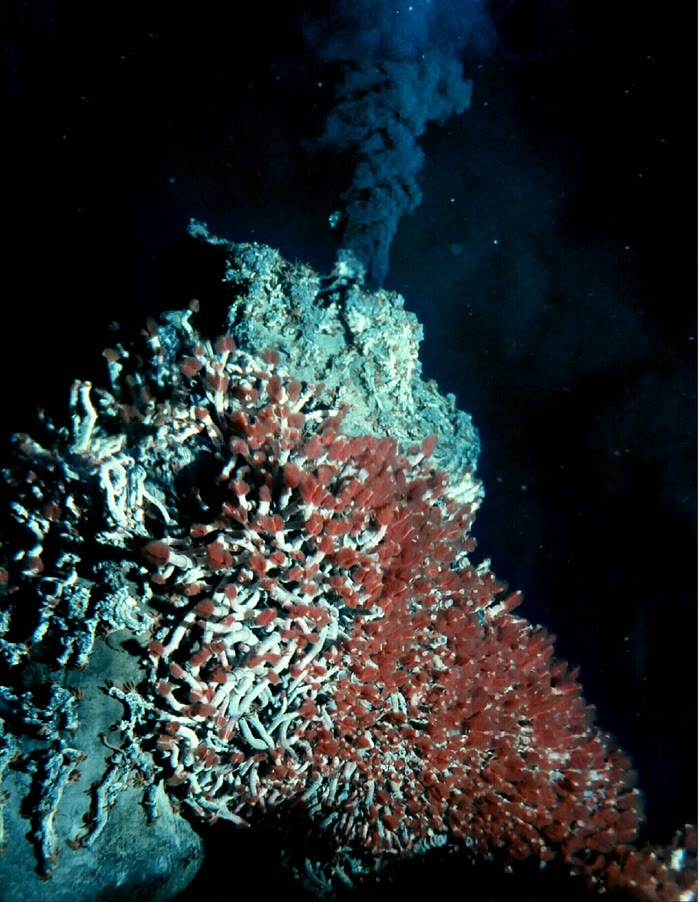
\includegraphics[width=\linewidth]{images/book2/g11-noaa-black-smoker.jpg}
\end{minipage}

{\small बाएँ: कटक-अक्ष पर \omterm{def:g11:ocean-ridges:hydrothermal}{जलतापीय परिसंचरण} (चित्र, पैमाने पर
नहीं)। दाएँ: ह्वान डी फ़्यूका कटक पर एक \omterm{def:g11:ocean-ridges:hydrothermal}{काला धूम्रक}, जिसकी चिमनी लाल गलफड़ों वाले
नलिका-कृमियों से ढकी है; फ़ोटो वॉशिंगटन विश्वविद्यालय और NOAA
(सार्वजनिक डोमेन)।}
\end{omfigure}
% ledger: whoi:vents, photo:g11-black-smoker

\begin{history}[गैलापागोस दरार पर \emph{ऐल्विन}, 1977]
राष्ट्रीय विज्ञान प्रतिष्ठान से वित्त-पोषित यह अभियान
8~फ़रवरी 1977 को शोध-जहाज़ \emph{नॉर} पर शुरू हुआ। कैमरा-स्लेज ऐंगस ने,
जिसे दरार के ऊपर \qty{2500}{m} नीचे खींचा गया, जल के तापमान में एक वृद्धि दर्ज की,
और उन्हीं चित्रों में उसकी फ़ोटो ने लावा पर सैकड़ों सफ़ेद
सीपियाँ और भूरे शंबुक-कवच दिखाए। \emph{ऐल्विन} के गोते 713 पर
भूवैज्ञानिक जैक कॉर्लिस और च्यर्ड वान ऐंडेल ने दरारों से \qty{8}{\celsius} पर
झिलमिलाता जल निकलता पाया, फिर \qty{17}{\celsius} तक, जबकि आसपास का गहरा
जल \qty{2}{\celsius} पर था; \qty{30}{cm} तक लंबी सफ़ेद सीपियाँ
लगभग \qty{50}{m} चौड़े क्षेत्र को ढके थीं। जहाज़ पर कोई जीवविज्ञानी नहीं था:
अभियान गरम जल के लिए आया था, और उसने जंतुओं का ऐसा समुदाय पाया जिसकी
किसी ने कल्पना नहीं की थी।
\end{history}
% ledger: whoi:alvin-1977

\section{ठंडा होना, मोटा होना, धँसना}

अक्ष से दूर जाते हुए \omterm{def:g11:lithosphere-asthenosphere:lithosphere}{स्थलमंडल} ऊपर से, अपने ऊपर के ठंडे महासागर के माध्यम से,
ठंडा होता है। ठंडी हुई परत समय के साथ मोटी होती जाती है:
\omterm{def:g11:lithosphere-asthenosphere:lithosphere}{स्थलमंडल} मोटा होता है, अक्ष पर कुछ किलोमीटर से पुरानी तली पर लगभग सौ
किलोमीटर तक। ठंडी चट्टान सिकुड़ती है और अधिक घनी हो जाती है, इसलिए
\omterm{def:g11:lithosphere-asthenosphere:lithosphere}{स्थलमंडल} \omterm{def:g11:lithosphere-asthenosphere:lithosphere}{दुर्बलतामंडल} पर अधिक नीचे तैरता है (\omterm{def:g11:lithosphere-asthenosphere:isostasy}{समस्थिति},
\cref{ch:g11:lithosphere-asthenosphere}): आयु बढ़ने के साथ महासागरीय तली धँसती है।
अपनी सतह से चालन द्वारा ठंडी होती किसी वस्तु के लिए
ठंडी हुई परत की मोटाई समय के वर्गमूल की तरह बढ़ती है।
% ledger: ps77:depth-age, rs09:lab

\begin{proposition}[महासागरीय तली की गहराई, उसकी आयु के सापेक्ष]\label{prop:g11:ocean-ridges:depth-age}
औसतन, आयु $t$ (मिलियन वर्षों में) की महासागरीय तली इस गहराई पर है:
\[
  d(t) = 2500 + 350\sqrt{t} \quad \text{मीटर} \qquad (0 \le t \le 70),
\]
और लगभग 20 मिलियन वर्ष से पुरानी तली के लिए,
\[
  d(t) = 6400 - 3200\,e^{-t/62.8} \quad \text{मीटर}:
\]
तली नई होने पर तेज़ी से धँसती है, फिर अधिकाधिक धीरे, लगभग
\qty{6400}{m} की ओर। (स्वीकृत: ये सूत्र 1977 में पार्सन्स और स्क्लेटर ने
उत्तरी प्रशांत और उत्तरी अटलांटिक की गहराइयों से, उनके
अवसादों के भार के लिए संशोधित करके, मिलाए थे।)
\end{proposition}
% ledger: ps77:depth-age

वर्गमूल नई तली को तेज़ी से धँसाता है: अपने पहले मिलियन वर्ष में
तली \qty{350}{m} धँसती है, अगले तीन मिलियन वर्षों में और
\qty{350}{m}, और 16 से 64 मिलियन वर्षों के बीच \qty{1400}{m}, उतना ही जितना
अपने पहले सोलह मिलियन वर्षों में। चरघातांकी नियम बताता है कि पुरानी
तली धँसना कैसे बंद करती है: वह ऐसे व्यवहार करती है मानो ठंडी होती प्लेट की एक नियत मोटाई हो,
लगभग \qty{125}{km}।
% ledger: ps77:depth-age

\begin{omfigure}
\begin{tikzpicture}
\begin{axis}[omrecord, omdepth, width=0.82\linewidth, height=6.2cm, xmin=0, xmax=180, ymin=2000, ymax=6600,
  xlabel={महासागरीय तली की आयु (मिलियन वर्ष)}, ylabel={गहराई (\unit{m})},
  yticklabel style={/pgf/number format/set thousands separator={}},
  legend style={font=\scriptsize, at={(0.5,-0.32)}, anchor=north, legend columns=3, /tikz/every even column/.append style={column sep=6pt}}, legend cell align=left]
% computed in figdata/grade-11/depth_age.py; ledger: data:etopo1, data:b2-seafloor-age, ps77:depth-age
\addplot[only marks, mark=*, mark size=1.3pt, black!70, error bars/.cd, y dir=both, y explicit]
  table[x=age, y=depth, y error minus=em, y error plus=ep] {figdata/out/grade-11-depth_age-bins.dat};
\addplot[omProp, line width=1.0pt] table[x=age, y=depth] {figdata/out/grade-11-depth_age-sqrt.dat};
\addplot[omDef, line width=1.0pt, densely dashed] table[x=age, y=depth] {figdata/out/grade-11-depth_age-exp.dat};
\legend{{मापित: माध्यिका और बीच का आधा भाग}, {$2500 + 350\sqrt{t}$}, {$6400 - 3200\,e^{-t/62.8}$}}
\end{axis}
\end{tikzpicture}

{\small महासागरीय तली की गहराई, उसकी आयु के सापेक्ष: हर 5 मिलियन वर्ष की आयु-पट्टी के लिए
संसार के महासागरों के सभी एक-अंश कोष्ठों की माध्यिका गहराई,
और उनके बीच के आधे भाग का परिसर। नई तली
वर्गमूल नियम का निकटता से अनुसरण करती है; पुरानी तली नियमों से उथली है, क्योंकि
उसके कोष्ठों में अवसाद और ज्वालामुखी शामिल हैं। आँकड़े: ETOPO1 (NOAA) और
सेटन और अन्य (2020) की महासागरीय तली की आयु; नियम पार्सन्स और स्क्लेटर के
(1977)।}
\end{omfigure}
% values (depth_age.py): median 2.5-5 Myr 3114 (law 3178), 60-65 Myr 4648 (law 5267), fit a 2727 b 255

नई तली की मापी गई गहराइयाँ नियम से लगभग
\qty{100}{m} के भीतर मेल खाती हैं। पुरानी तली पर मापी गई माध्यिकाएँ नियमों से कई सौ मीटर
ऊपर हैं। नियम स्वयं तली की गहराई बताते हैं, मानो उसके
अवसाद हटा दिए गए हों; मापे गए कोष्ठों में अब भी उनके अवसाद हैं,
जो तली की आयु के साथ अधिक मोटे होते हैं और पश्चिमी उत्तरी अटलांटिक की सबसे पुरानी तली पर
एक किलोमीटर से अधिक मोटे हैं, और उनमें
समुद्री पर्वत और ज्वालामुखीय पठार भी शामिल हैं।
% ledger: ps77:depth-age; values from depth_age.py

इसलिए पुराना \omterm{def:g11:ocean-ridges:oceanic-lithosphere}{महासागरीय स्थलमंडल} मोटा, ठंडा और घना है। अगला अध्याय
दिखाता है कि वह अपने नीचे के \omterm{def:g11:lithosphere-asthenosphere:lithosphere}{दुर्बलतामंडल} से अधिक घना हो सकता है, और
वापस प्रावार में डूब सकता है (\cref{ch:g11:subduction-zones})।

\section{अभ्यास}

\begin{exercise}[$\star$]\label{exo:g11:ocean-ridges:1}
\omterm{def:g11:ocean-ridges:peridotite}{पेरिडोटाइट} और \omterm{def:g11:ocean-ridges:gabbro}{गैब्रो} की परिभाषा दीजिए। दोनों में से कौन \omterm{def:g11:ocean-ridges:oceanic-lithosphere}{महासागरीय भूपर्पटी} का अंग है,
और कौन प्रावार का? \omterm{def:g11:ocean-ridges:gabbro}{गैब्रो} का संघटन बेसाल्ट जैसा ही है: उसके
क्रिस्टल इतने अधिक बड़े क्यों हैं?
\end{exercise}

\begin{exercise}[$\star$]\label{exo:g11:ocean-ridges:2}
समुद्री तल से नीचे की ओर \omterm{def:g11:ocean-ridges:oceanic-lithosphere}{महासागरीय स्थलमंडल} की परतों की सूची बनाइए। पूर्वी
प्रशांत का गहरा छेद समुद्री तल से \qty{1507}{m} नीचे तक पहुँचा: उसने
\qty{7.1}{km} की भूपर्पटी का कितना भाग पार किया?
\end{exercise}

\begin{exercise}[$\star$]\label{exo:g11:ocean-ridges:3}
$d = 2500 + 350\sqrt{t}$ का उपयोग करके 0, 9 और 25
मिलियन वर्ष पुरानी महासागरीय तली की गहराई ज्ञात कीजिए।
\end{exercise}

\begin{exercise}[$\star$]\label{exo:g11:ocean-ridges:4}
\omterm{def:g11:ocean-ridges:normal-fault}{सामान्य भ्रंश} की परिभाषा दीजिए। किसी धीमे कटक पर कौन-सा बल \omterm{def:g11:ocean-ridges:normal-fault}{सामान्य भ्रंश} बनाता है, और
भ्रंशों के ऊपर के खंड किस दिशा में चलते हैं?
\end{exercise}

\begin{exercise}[$\star$]\label{exo:g11:ocean-ridges:5}
काले धूम्रक का जल लगभग \qty{350}{\celsius} पर निकलता है। वह
उबलता क्यों नहीं? काला ``धुआँ'' क्या है?
\end{exercise}

\begin{exercise}[$\star\star$]\label{exo:g11:ocean-ridges:6}
गलन वाले चित्र का उपयोग कीजिए: (1) \qty{1300}{\celsius} विभव
ताप वाला प्रावार किस गहराई पर पिघलना शुरू करता है, और किस तापमान पर? (2)
और उससे \qty{100}{\celsius} अधिक गरम प्रावार? (3) दोनों में से कौन
अधिक मोटी भूपर्पटी बनाता है? क्यों?
\end{exercise}

\begin{exercise}[$\star\star$]\label{exo:g11:ocean-ridges:7}
\qty{1300}{\celsius} विभव ताप वाली ऊपर उठती प्रावार-चट्टान \qty{100}{km} की गहराई पर
\qty{1345}{\celsius} पर है, जहाँ उसका
गलनांक \qty{1489}{\celsius} है। (1) वह अपने गलनांक से
कितना नीचे है? (2) वह \qty{54}{km} पर पिघलना शुरू करती है। ऊपर जाते हुए
औसतन प्रति किलोमीटर कितने अंश यह अंतर घटा है? (3) क्या चट्टान को
गरम किया गया है?
\end{exercise}

\begin{exercise}[$\star\star$]\label{exo:g11:ocean-ridges:8}
\ang{30} दक्षिण पर पूर्वी प्रशांत उभार प्रति वर्ष \qty{14.6}{cm} खुलता है,
मध्य-अटलांटिक कटक प्रति वर्ष \qty{3.3}{cm}। सममित प्रसरण मानकर बताइए कि हर कटक को
एक ओर \qty{1000}{km} तली बनाने में कितना समय लगता है।
\end{exercise}

\begin{exercise}[$\star\star$]\label{exo:g11:ocean-ridges:9}
कटक लगभग \qty{65000}{km} लंबे हैं। मान लीजिए वे औसतन
प्रति वर्ष \qty{5}{cm} खुलते हैं और \qty{7.1}{km} मोटी भूपर्पटी बनाते हैं। (1) वे हर वर्ष
कितने क्षेत्रफल की नई महासागरीय तली बनाते हैं? (2) भूपर्पटी का कितना आयतन? (3) महासागरों के क्षेत्रफल,
\qty{3.6e8}{km^2}, के बराबर क्षेत्रफल बनाने में उन्हें कितना समय लगेगा?
\end{exercise}

\begin{exercise}[$\star\star$]\label{exo:g11:ocean-ridges:10}
एक अक्षीय घाटी \qty{1.5}{km} गहरी है। वह आमने-सामने के दो \omterm{def:g11:ocean-ridges:normal-fault}{सामान्य भ्रंशों} के अनुदिश
धँसी, हर एक \ang{60} पर झुका। (1) हर भ्रंश
अपने तल के अनुदिश कितना खिसका? (2) दोनों भ्रंशों के कारण दोनों ओर क्षैतिज रूप से
एक-दूसरे से कितनी दूर हुए? (3) घाटी \qty{25}{km} चौड़ी है: क्या उसे
केवल भ्रंशन ने बनाया?
\end{exercise}

\begin{exercise}[$\star\star$]\label{exo:g11:ocean-ridges:11}
$d = 6400 - 3200\,e^{-t/62.8}$ का उपयोग करके 25 और 100
मिलियन वर्ष पुरानी तली की गहराई ज्ञात कीजिए, और यह कि इन आयुओं के बीच तली कितना धँसती है। पहले
मान की तुलना वर्गमूल नियम के मान से कीजिए।
\end{exercise}

\begin{exercise}[$\star\star\star$]\label{exo:g11:ocean-ridges:12}
प्रावार का \qty{100}{km} मोटा एक स्तंभ औसतन \qty{700}{\celsius}
ठंडा होता है। चट्टान ठंडा होने के हर अंश पर अपनी लंबाई का $\alpha = 3.2 \times 10^{-5}$
सिकुड़ती है। (1) स्तंभ कितना छोटा होता है? (2) जैसे-जैसे वह
धँसता है, समुद्री जल (\qty{1025}{kg/m^3}) उसके ऊपर का स्थान भर देता है; \qty{3380}{kg/m^3} के
प्रावार-घनत्व के साथ \omterm{def:g11:lithosphere-asthenosphere:isostasy}{समस्थिति} तली को
$s = \rho_m\,\alpha\,\Delta T\,L/(\rho_m - \rho_w)$ धँसाती है। $s$ परिकलित कीजिए। (3) इसकी तुलना
उस कुल धँसाव से कीजिए जिसकी चरघातांकी नियम अनुमति देता है, \qty{2500}{m} से
\qty{6400}{m} तक।
\end{exercise}

\begin{exercise}[$\star\star\star$]\label{exo:g11:ocean-ridges:13}
\qty{1300}{\celsius} वाले प्रावार में गलन \qty{54}{km} नीचे शुरू होता है,
\qty{1400}{\celsius} वाले में \qty{85}{km} नीचे; दोनों में गलन
भूपर्पटी के आधार तक, लगभग \qty{7}{km} नीचे तक, चलता रहता है। (1) दोनों गलन-स्तंभों की
लंबाइयों की तुलना कीजिए। (2) यदि ऊपर उठती चट्टान का हर किलोमीटर उतना ही
पिघला पदार्थ देता, तो सामान्य प्रावार के ऊपर \qty{7.1}{km} की भूपर्पटी के लिए, अधिक गरम प्रावार के ऊपर
भूपर्पटी कितनी मोटी होती? (3) जहाँ कटक अधिक गरम प्रावार से मिलते हैं, वहाँ मापी गई
\qty{10.3}{km} से तुलना कीजिए।
\end{exercise}

\begin{exercise}[$\star\star\star$]\label{exo:g11:ocean-ridges:14}
महासागरीय तली की मापी गई माध्यिका गहराइयाँ \num{3.75} मिलियन वर्ष की आयु पर \qty{3114}{m},
\num{22.5} पर \qty{4018}{m}, \num{42.5} पर \qty{4465}{m}
और \num{62.5} पर \qty{4648}{m} हैं। (1) हर आयु पर वर्गमूल नियम द्वारा दी गई
गहराई, और मापन से उसका अंतर, परिकलित कीजिए। (2)
आयु के साथ अंतर कैसे बदलता है? (3) इसे समझाइए।
\end{exercise}

\begin{exercise}[$\star\star\star$]\label{exo:g11:ocean-ridges:15}
जल का क्रांतिक बिंदु \qty{374}{\celsius} और \qty{22.064}{MPa} पर है: उस दाब से
ऊपर जल किसी भी तापमान पर नहीं उबलता। (1) \qty{2500}{m} नीचे जल का
दाब परिकलित कीजिए (समुद्री जल \qty{1025}{kg/m^3},
$g = \qty{9.8}{m/s^2}$, और वायुमंडल का \qty{0.1}{MPa})। (2) क्या उस गहराई पर किसी निकास का
जल उबल सकता है, चाहे वह कितना भी गरम हो? (3) लगभग किस
गहराई के नीचे यह हर निकास के लिए सच है?
\end{exercise}

\section{समस्या: प्रशांत तली के एक टुकड़े का जीवन}

\begin{problem}[{सप्ताहांत समस्या --- कटक से गहरे महासागर तक}]
\label{pb:g11:ocean-ridges:1}
% values: EPR 30 S full rate 145.8 mm/yr (plate_velocities.py, nnr56:poles); depth law
% ps77:depth-age; crust white92:crust; alpha ps77; densities data:prem; median 60-65 Myr
% 4648 m (depth_age.py)
महासागरीय तली का एक टुकड़ा आज \ang{30} दक्षिण पर पूर्वी प्रशांत उभार पर जन्म लेता है,
जहाँ प्रशांत और नाज़्का प्लेटें प्रति वर्ष \qty{14.6}{cm} की दर से एक-दूसरे से दूर होती हैं।
वह प्रशांत प्लेट के साथ पश्चिम की ओर चलता है। प्रसरण को सममित,
भूपर्पटी को \qty{7.1}{km} मोटी, और गहराई का नियम $d = 2500 + 350\sqrt{t}$ मीटर
लीजिए ($t$ मिलियन वर्षों में)।

\medskip
\noindent\textbf{भाग I --- कटक पर जन्म।}
\begin{enumerate}
  \item अर्ध \omterm{def:g11:drift-to-spreading:spreading-rate}{प्रसरण दर} क्या है, सेंटीमीटर प्रति वर्ष में और
        किलोमीटर प्रति मिलियन वर्ष में?
  \item तली का यह टुकड़ा किस गहराई पर जन्म लेता है?
  \item समुद्री तल से \omterm{def:g11:lithosphere-asthenosphere:lithosphere}{स्थलमंडल} के आधार तक, वह जिन चट्टानों से बना है उनकी
        सूची बनाइए।
  \item जिस मैग्मा ने उसे बनाया, वह नीचे के प्रावार से आया। समझाइए कि
        प्रावार बिना गरम किए कैसे पिघला।
  \item यह कटक अपनी लंबाई के हर किलोमीटर के लिए, दोनों ओर, हर मिलियन वर्ष में
        भूपर्पटी का कितना आयतन बनाता है?
\end{enumerate}

\medskip
\noindent\textbf{भाग II --- यात्रा।}
\begin{enumerate}[resume]
  \item यदि दर वैसी ही रहे, तो 1, 4, 16 और 64
        मिलियन वर्ष बाद टुकड़ा कटक से कितनी दूर होगा?
  \item \qty{2000}{km} की यात्रा करने में उसे कितना समय लगेगा?
  \item 64 मिलियन वर्ष बाद की वास्तविक दूरी प्रश्न~6 के
        उत्तर से भिन्न क्यों हो सकती है?
  \item कटक के पास समुद्री जल नई भूपर्पटी से होकर परिसंचरित होता है और
        निकासों पर बाहर आता है। पुरानी तली पर यह परिसंचरण क्यों रुक जाता है?
  \item टुकड़ा किस प्लेट पर यात्रा करता है, और वह प्लेट उसे अपनी पश्चिमी ओर
        किस प्रकार की प्लेट-सीमा की ओर ले जाती है?
\end{enumerate}

\medskip
\noindent\textbf{भाग III --- आयु के साथ धँसना।}
\begin{enumerate}[resume]
  \item 1, 4, 16 और 64 मिलियन वर्ष पर उसकी गहराई परिकलित कीजिए।
  \item अपने पहले 16 मिलियन वर्षों में, और 16 से 64 मिलियन वर्षों के बीच,
        वह कितना धँसता है? टिप्पणी कीजिए।
  \item वह किस आयु पर \qty{4000}{m} की गहराई तक पहुँचता है?
  \item 64 मिलियन वर्ष पर उसकी गहराई की तुलना चरघातांकी नियम,
        $6400 - 3200\,e^{-t/62.8}$, से कीजिए।
  \item 60 से 65 मिलियन वर्ष पुरानी महासागरीय तली की मापी गई माध्यिका गहराई
        \qty{4648}{m} है। अंतर समझाइए।
\end{enumerate}

\medskip
\noindent\textbf{भाग IV --- उसका घनत्व और उसकी नियति।}
\begin{enumerate}[resume]
  \item 64 मिलियन वर्ष तक उसके \omterm{def:g11:lithosphere-asthenosphere:lithosphere}{स्थलमंडल} को \qty{100}{km} मोटा और
        \omterm{def:g11:lithosphere-asthenosphere:lithosphere}{दुर्बलतामंडल} से औसतन \qty{700}{\celsius} ठंडा लीजिए।
        प्रति अंश $\alpha = 3.2 \times 10^{-5}$ के साथ,
        प्रावार-भाग कितने भिन्न से अधिक घना हुआ है? \qty{3380}{kg/m^3} से आरंभ करके,
        उसका घनत्व क्या है?
  \item उसकी भूपर्पटी \qty{7.1}{km} मोटी है, जिसका घनत्व
        \qty{2900}{kg/m^3} है। \omterm{def:g11:lithosphere-asthenosphere:lithosphere}{स्थलमंडल} के पूरे
        \qty{100}{km} का माध्य घनत्व परिकलित कीजिए।
  \item उसके नीचे के \omterm{def:g11:lithosphere-asthenosphere:lithosphere}{दुर्बलतामंडल} से तुलना कीजिए, जिसे
        \qty{3380}{kg/m^3} लिया गया है।
  \item किसी खाई तक पहुँचने पर ऐसा \omterm{def:g11:lithosphere-asthenosphere:lithosphere}{स्थलमंडल} क्या कर सकता है?
  \item निष्कर्ष निकालिए: 64 मिलियन वर्ष का होने पर तली का यह टुकड़ा
        किस गहराई पर है?
\end{enumerate}
\end{problem}
